\documentclass[12pt,letterpaper]{article}
\usepackage[utf8]{inputenc}
\usepackage{amsmath}
\usepackage{amsfonts}
\usepackage{amssymb}
\usepackage{amsthm}
\usepackage{graphicx}
\usepackage{tabularx}
\usepackage[left=2cm,right=2cm,top=2cm,bottom=2cm]{geometry}
\usepackage{multicol}
\usepackage{lastpage}
\usepackage{fancyhdr}
\usepackage{multirow,array}
\usepackage{newtxtext,newtxmath}
\usepackage{lastpage}
\usepackage{enumitem}
\newcolumntype{Y}{>{\centering\arraybackslash}X}
\pagestyle{fancy}
\fancyhf{}
\lhead{\textsc{BHCC Mat-181}}
\chead{\textsc{Answers}}
\rhead{\textsc{HW Exercises 2.1-2.8}}
\rfoot{Page \thepage ~of \pageref{LastPage}}
\setenumerate[1]{label={\bf 2.\theenumi: }}
\setenumerate[2]{label={\bf (\theenumii): }}
\setenumerate[3]{label={\bf \theenumiii: }}

\begin{document}
\begin{enumerate}
%\setcounter{enumi}{68}
\item \begin{enumerate}
    \item False. Each toss has a 50\% chance of landing heads.
    \item False. You can draw a red face card, like the queen of hearts.
    \item True, because an ace card is not a face card (even though we pretended otherwise for the gender discrimination simulations).
\end{enumerate}

\item \begin{enumerate}
    \item $P(\rm{red}) = \frac{18}{38} \approx 0.47$
    \item Well, if we assume the wheel is fair, then $P(\rm{red}) = \frac{18}{38} \approx 0.47$. (See part (c).)
    \item Haha! Not really. 300 consecutive reds seems rather fishy. 
\end{enumerate}

\item \begin{enumerate}
    \item 10. We want the sample proportion $\hat{p}$ to be far from the probability, which is 0.5. Thus, we want a small sample size. Large samples will have sample proportions near the probability.
    \item 100. We want the sample proportion to be near 0.5.
    \item 100. We want the sample proportion to be near 0.5.
    \item 10. We want the sample propotion far from 0.5.
\end{enumerate}

\item I rolled four 6s in a row. The probability of this can be determined using the product rule for indepenedent events.
$$P(\text{four 6s}) = P(\text{first is 6}) \times P(\text{second is 6})\times P(\text{third is 6})\times P(\text{fourth is 6})$$
$$P(\text{four 6s}) = \left(\frac{1}{6}\right)^4 = \frac{1}{1296} \approx 0.00077$$
My friend rolled four 3s in a row.
$$P(\text{four 3s}) = P(\text{first is 3}) \times P(\text{second is 3})\times P(\text{third is 3})\times P(\text{fourth is 3})$$
$$P(\text{four 3s}) = \left(\frac{1}{6}\right)^4 = \frac{1}{1296} \approx 0.00077$$

You might also consider the following:\\
 When rolling two dice, there are 36 possible equally likely outcomes.
\begin{center}
\begin{tabular}{|c c|c c c c c c|}\hline
            &   & \multicolumn{6}{|c|}{first die} \\
            &   & 1 & 2 & 3 & 4 & 5 & 6 \\ \hline
            &1  &1,1&2,1&3,1&4,1&5,1&6,1\\
            &2  &1,2&2,2&3,2&4,2&5,2&6,2\\
second die  &3  &1,3&2,3&3,3&4,3&5,3&6,3\\
            &4  &1,4&2,4&3,4&4,4&5,4&6,4\\
            &5  &1,5&2,5&3,5&4,5&5,5&6,5\\
            &6  &1,6&2,6&3,6&4,6&5,6&6,6\\ \hline
\end{tabular}
\end{center}
This means that on each turn, a player has a $\frac{1}{36}$ chance to roll two 3s. On each turn, a player has the same chance to roll two 6s. Then, the chance to do two 3s twice can be determined using the multiplication rule. Let $A$ mean a double on first turn and let $B$ mean the same double on the second turn.
$$P(A~\rm{and}~B) = P(A)\times P(B|A)$$
Because each turn is independent, we know $P(B|A)=P(B)$. Thus,
$$P(A~\rm{and}~B) = \frac{1}{36} \times \frac{1}{36}$$

\item \begin{enumerate}
\item $P(\text{ten tails}) = \left(\frac{1}{2}\right)^{10} = \frac{1}{1024} \approx 0.00098$
\item $P(\text{ten heads}) = \left(\frac{1}{2}\right)^{10} = \frac{1}{1024} \approx 0.00098$
\item We can use complementary events here. The events ``ten heads'' and ``at least one tails'' are complementary, so they should sum to 1.
\begin{align*}
P(\text{at least one tails}) &= 1-P(\text{ten heads}) \\
&= 1- \frac{1}{1024} \\
&= \frac{1023}{1024} \\
&\approx 0.999
\end{align*}
\end{enumerate}

\item \begin{enumerate}
\item 0. It is impossible for two dice to sum to 1.
\item When rolling two dice, there are 36 equally-likely outcomes, 4 of which are favorable to the event: 
%$$\{1,4 ~~;~~ 2,3 ~~;~~ 3,2 ~~;~~ 4,1 \}$$

\begin{center}
\begin{tabular}{|c c|c c c c c c|}\hline
            &   & \multicolumn{6}{|c|}{first die} \\
            &   & 1 & 2 & 3 & 4 & 5 & 6 \\ \hline
            &1  &1,1&2,1&3,1&\bf 4,1&5,1&6,1\\
            &2  &1,2&2,2&\bf 3,2&4,2&5,2&6,2\\
second die  &3  &1,3&\bf 2,3&3,3&4,3&5,3&6,3\\
            &4  &\bf 1,4&2,4&3,4&4,4&5,4&6,4\\
            &5  &1,5&2,5&3,5&4,5&5,5&6,5\\
            &6  &1,6&2,6&3,6&4,6&5,6&6,6\\ \hline
\end{tabular}
\end{center}
So, $P(\text{sum of 5}) = \frac{4}{36} \approx 0.1111$
\item There is only one (of 36) ways to roll a sum of 12.
$$P(\text{sum of 12}) = \frac{1}{36} \approx 0.0278 $$
\end{enumerate}

\item \begin{enumerate}
\item Nope. Some voters are both.
\item ~\\ 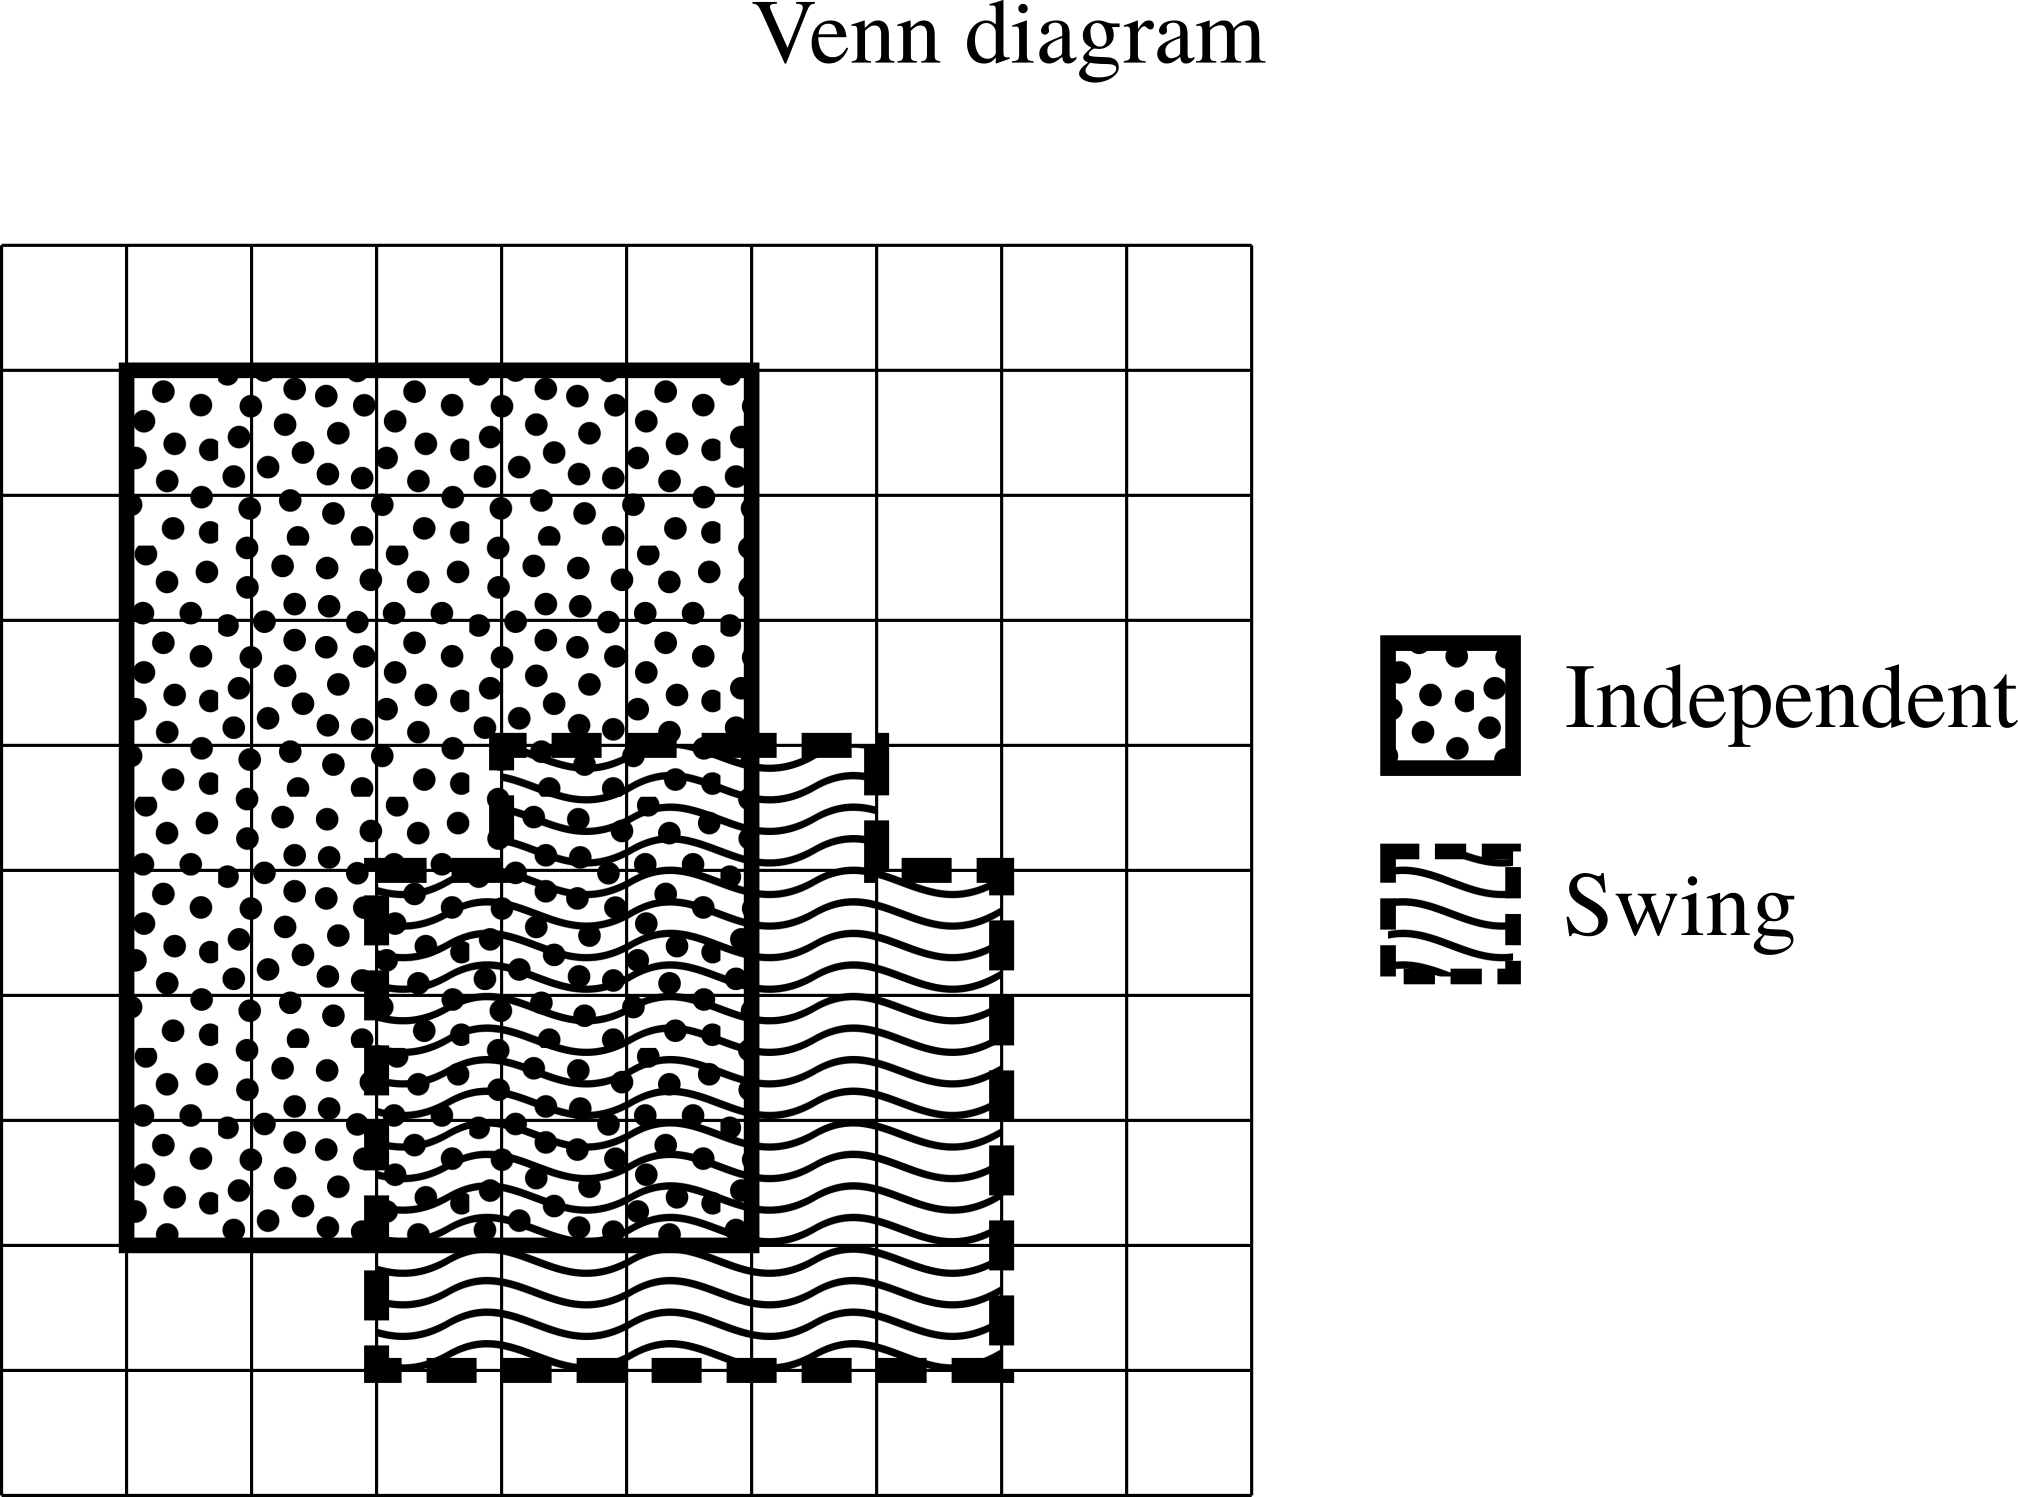
\includegraphics[scale=0.6]{figures/venn.png}
\\
Or, we could do the following:~\\ 
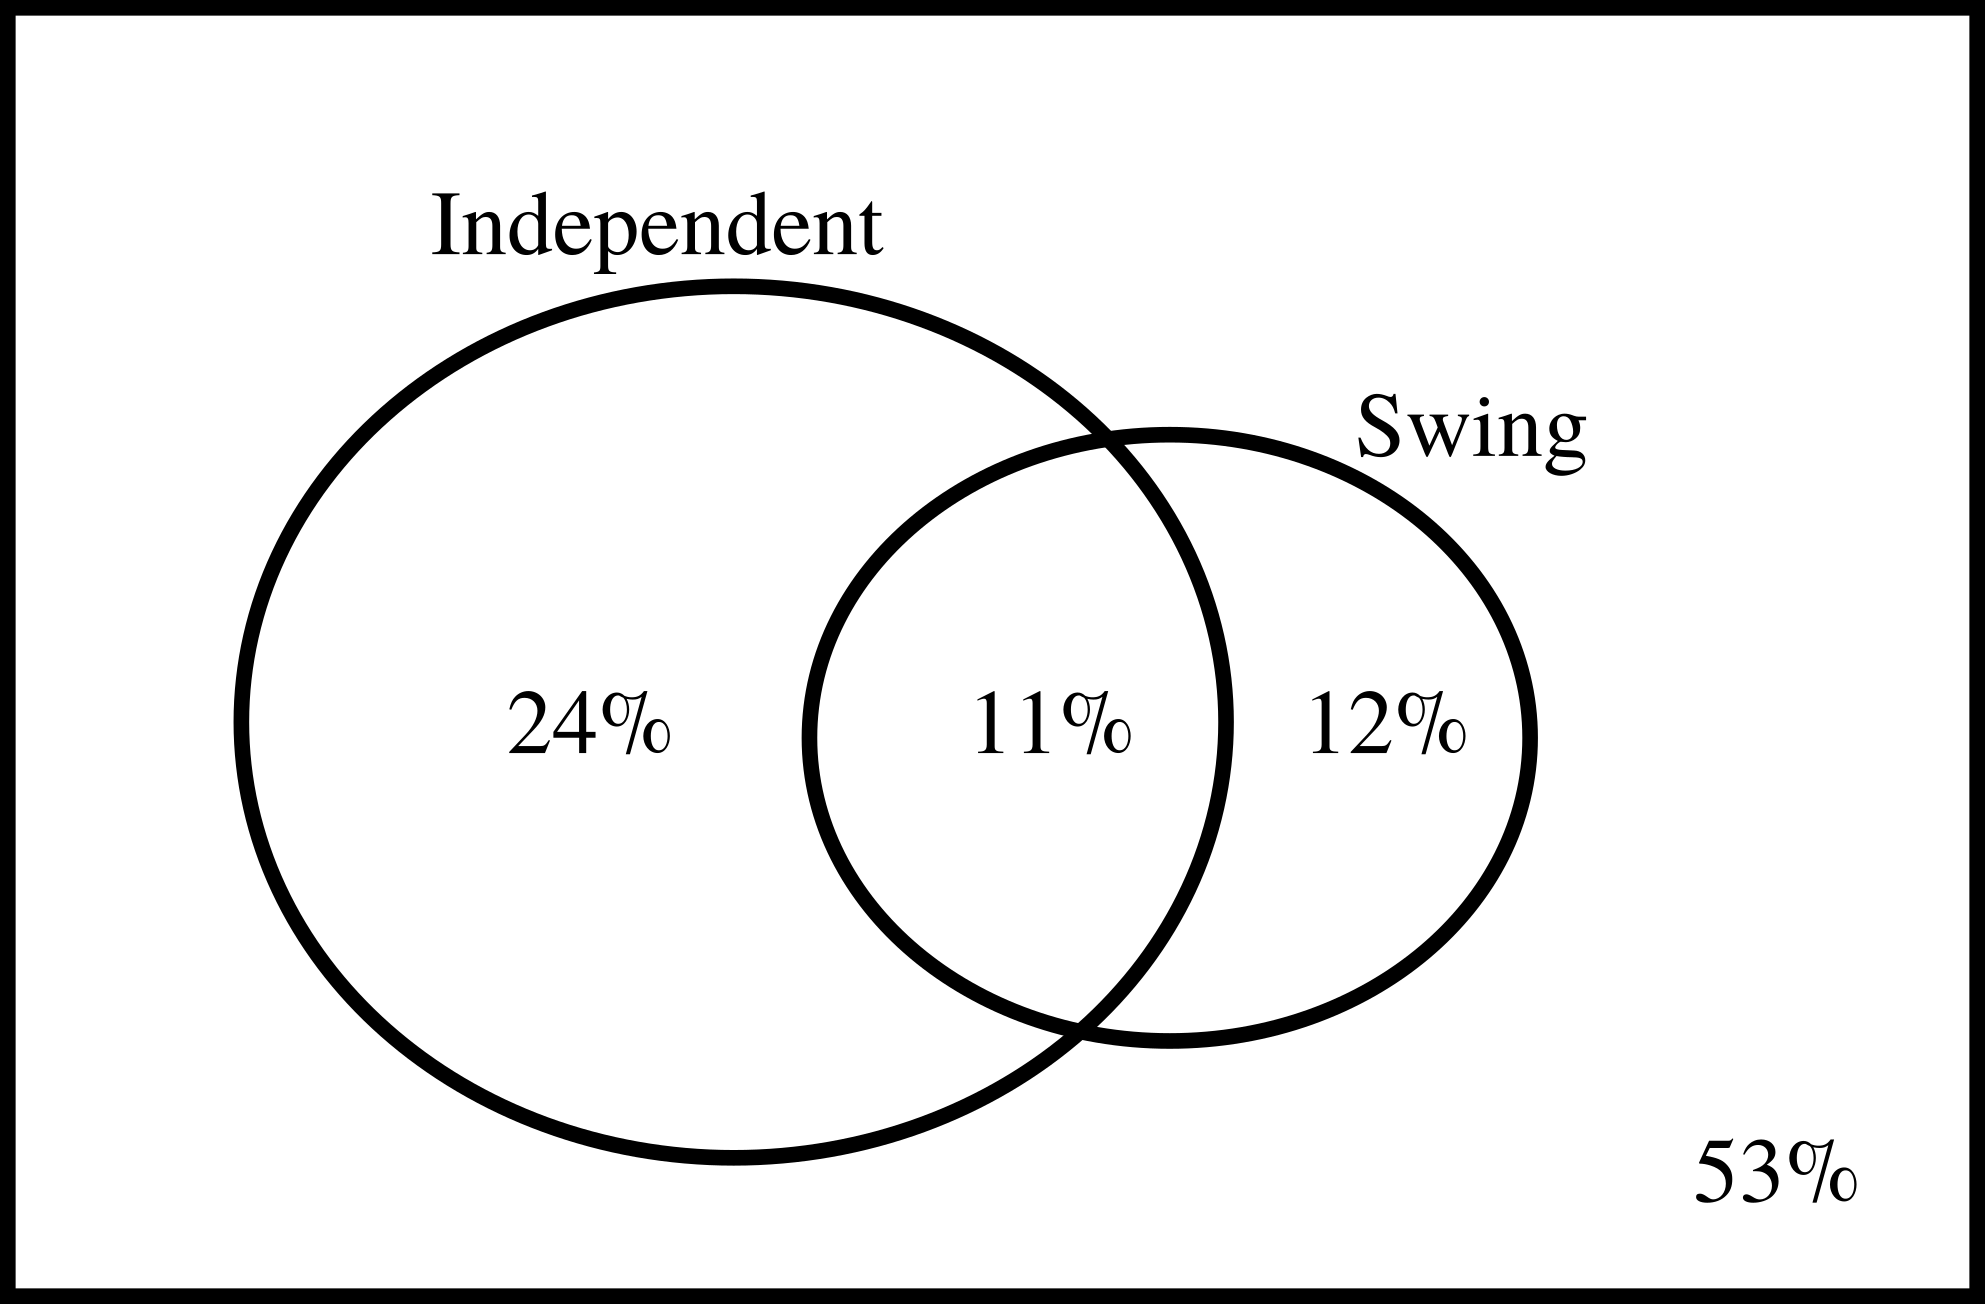
\includegraphics[scale=0.5]{figures/venn2.png}
\\
Also, if you interpreted the prompt to mean 35\% were only independent, 23\% were only swing, and 11\% were both, I'd understand why you interpreted it that way.
\item 24\%
\item 47\%
\item 53\%
\item Wow, this is confusing... we are using ``Independent'' for political affiliation and ``independent'' for probability concept. 
\\
$P(\text{swing}|\text{Independent}) = \frac{11}{35} \approx 0.314$
\\
$P(\text{swing}|\text{not Independent}) = \frac{12}{65} \approx 0.185$
\\
$P(\text{swing}) = \frac{23}{100} = 0.23$
\\
Because $P(\text{swing}|\text{Independent}) \ne P(\text{swing})$, swingness is dependent on Independentness.

Also, we could have used the other test of independence.
$$\text{independence} ~~\iff~~ P(A~\text{and}~B) = P(A)\times P(B)$$

$$P(Indy~\text{and}~swing) = 0.11$$
$$P(Indy) = 0.35$$
$$P(swing) = 0.23$$
$$P(Indy)\times P(swing) = 0.0805 $$
$$P(Indy~\text{and}~swing) \ne P(Indy)\times P(swing)$$
So, swingness is dependent on Independentness.
\end{enumerate}

\item \begin{enumerate}
\item Nope.
\item ~\\ 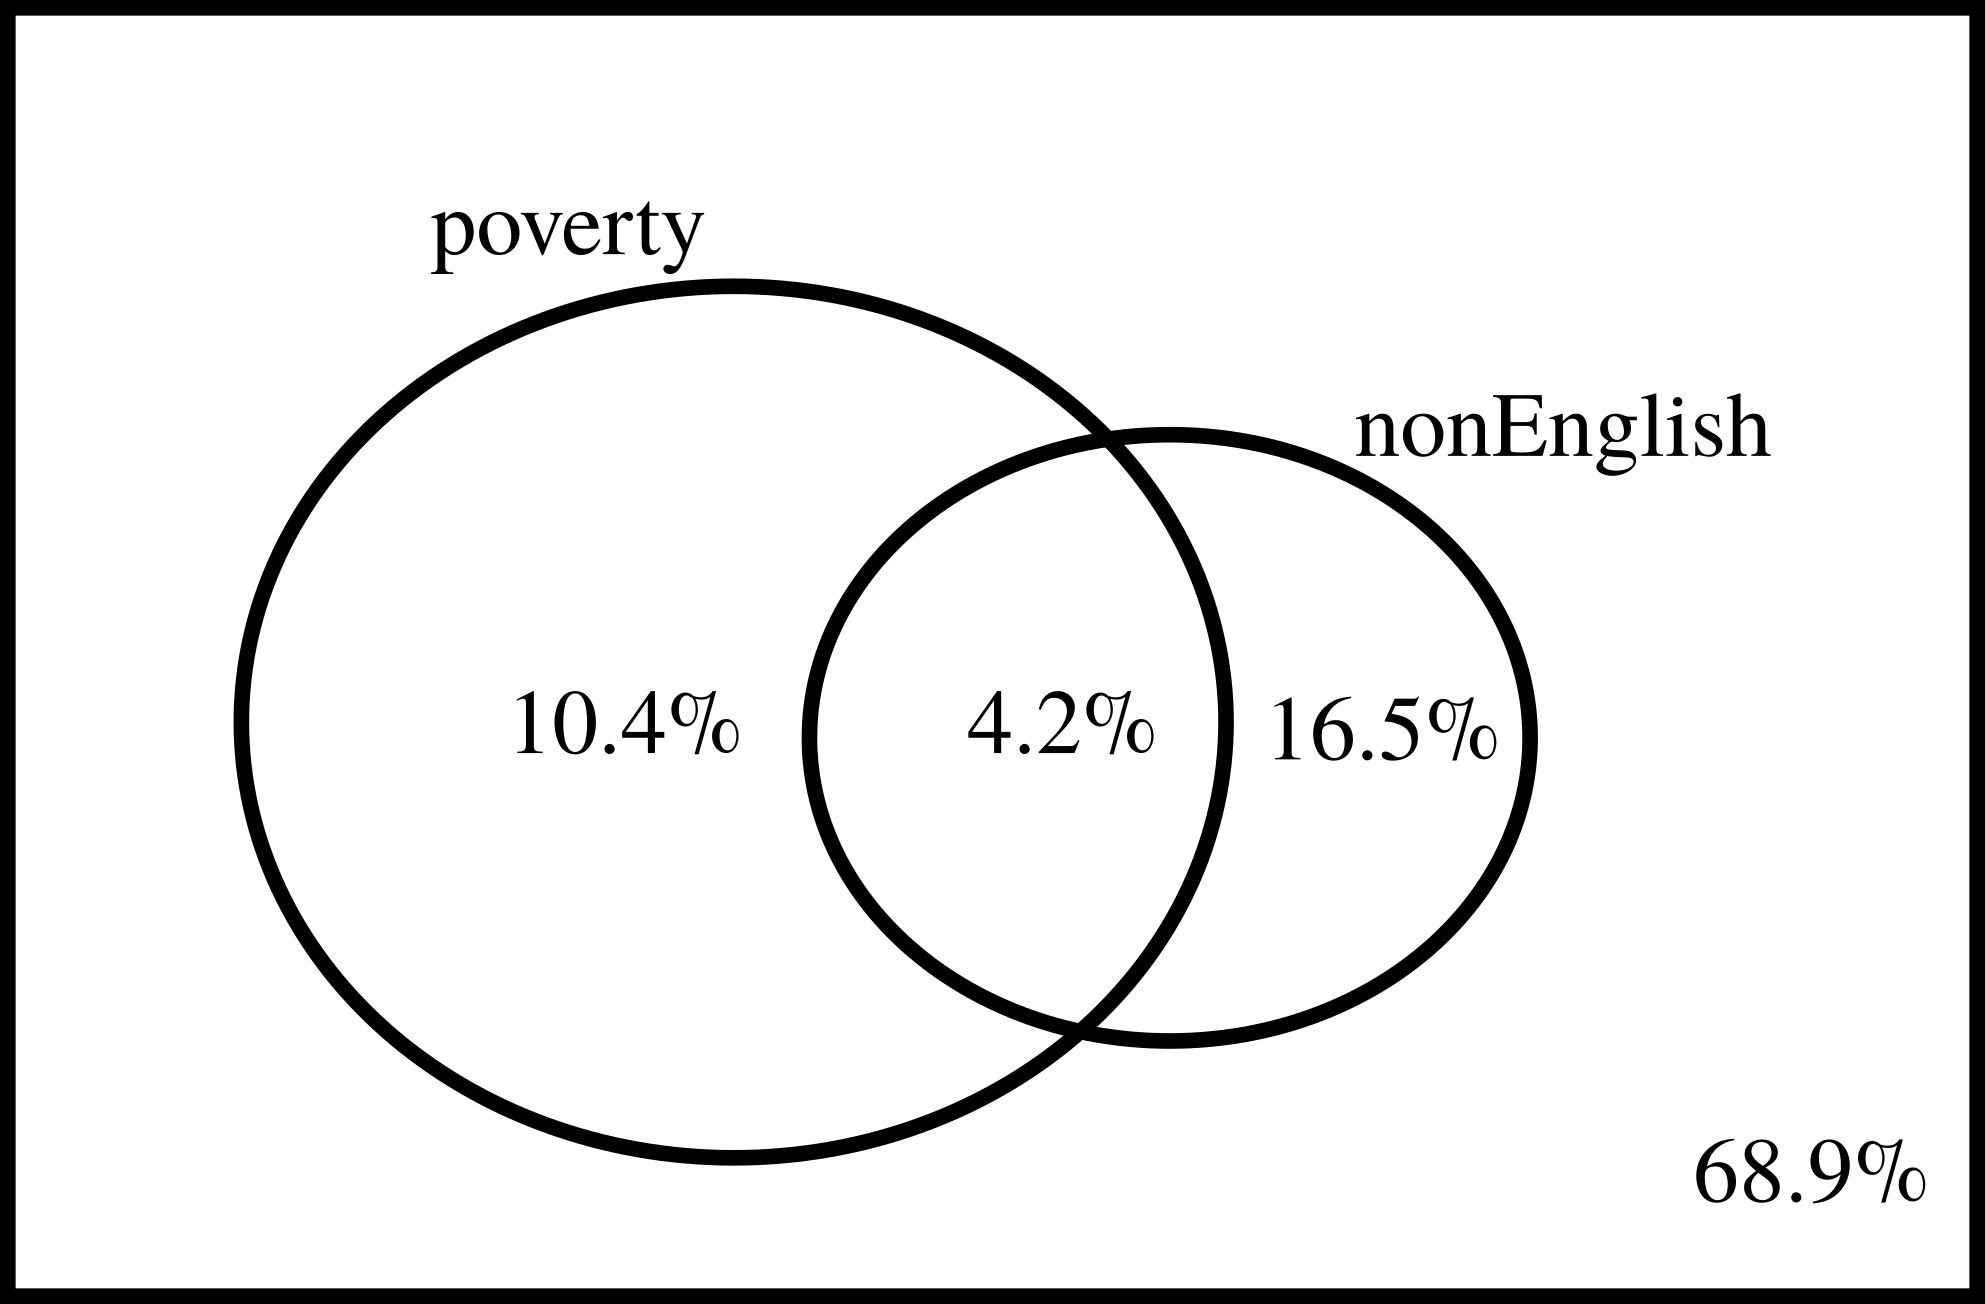
\includegraphics[scale=0.4]{figures/venn3.png}
\item 10.4\%
\item 31.1\%
\item 68.9\%
\item $$P(\text{poverty}) = 0.146$$
$$P(\text{nonEnglish}) = 0.207$$
$$P(\text{poverty and nonEnglish}) = 0.042$$
$$P(\text{poverty}) \times P(\text{nonEnglish}) \approx 0.146\times 0.207 \approx 0.03 \ne 0.042 $$
No. The events are dependent.
\end{enumerate}

\end{enumerate}
\end{document}
